\chapter{Choix des composants}


\section{Antennes}

\subsubsection{Principes généraux}

	Les goniomètres utilisent les ondes radioélectriques pour pouvoir localiser la direction d'une source d'émissions. Chaque type de goniomètre utilisera une ou plusieurs antennes pour pouvoir analyser les caractéristiques de l'onde reçue. 
	Le fonctionnement de ces antennes est décrit par les lois de l'électromagnétisme. Chaque onde électromagnétique possède une composante électrique et une composante magnétique. La composante ou champ électrique de cette onde fera apparaitre des variations de potentiel dans l'antenne dont l'amplitude et la fréquence seront directement liés à l'onde qui les a généré. Leur analyse permettra de récupérer les caractéristiques de l'onde reçue et d'en extraire les informations pertinentes pour le système équipé de l'antenne.

        \begin{center}
          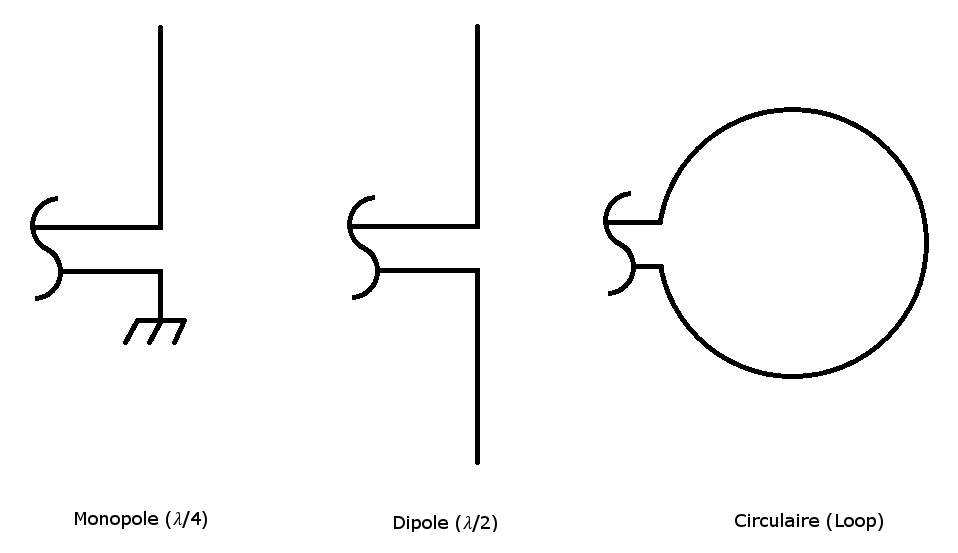
\includegraphics[width=0.8\textwidth]{antennes}
          \captionof{figure}{Type d'antennes}
        \end{center}

\subsection{Antennes en Radiogoniométrie}

En radiogoniométrie il est possible de travailler avec plusieurs types d'antennes. La méthode la plus simple pour déterminer la direction d'une onde sera d'utiliser une antenne à ouverture dite faible et de la faire pivoter pour pouvoir déterminer la direction du maximum d'émission. Une antenne circulaire ou rectangulaire pourra convenir. Parfois le type de goniomètre utilisé déterminera le choix de l'antenne. Par exemple dans le cas d'un radiogoniomètre de type Watson-Watt\footnote{principe décrit en \ref{Watson-Watt} à la page \pageref{Watson-Watt}} plusieurs solutions sont envisageables: 
	
\begin{itemize}

\item l'utilisation de deux antennes circulaires ou rectangulaires.

\item L'utilisation d'une antenne dite "Adcock" qui est une combinaison d'antennes monopoles ou dipolaires. 

\end{itemize} 

	Dans le cadre de notre projet, nos recherches nous ont conduit à choisir un goniomètre Doppler. Ce type de goniomètre utilise au minimum quatres antennes monopoles ou dipolaires disposées en croix autour d'une antennes de référence omnidirectionnelle (une antenne monopole est souvent utilisée). Pour un nombre d'antennes supérieur celles-ci seront disposées en cercle à intervalle régulier autour de l'antenne de référence.	
	
	En théorie deux antennes pourraient suffire. Si on parvenait à mettre en rotation une antenne omnidirectionelle autour de l'antenne de référence suffisamment rapidement le goniomètre Doppler fonctionnerait. Il est toutefois beaucoup plus simple d'utiliser un ensemble d'antennes disposées en cercle et "d'écouter" successivement chaque antenne à l'aide d'un commutateur pour simuler cette rotation.
	
\subsection{Système d'antennes retenu}

	Le goniomètre Montréal possède cinq antennes, quatre disposées en croix et une antenne centrale connectées au système électronique de traitement. Les antennes sont reliées à un commutateur permettant de sélectionner successivement les antennes de la croix. Le système est dimensionné autour de trois critères : 
	
\begin{itemize}

\item La bande de fréquence surveillée par les antennes : On utilisera ici des antennes monopoles (quart d'onde) adaptées au 2,4GHz

\item Le rayon d'écartement des antennes (distance entre les quatres antennes de la croix et l'antenne de référence) : Si ce rayon est trop faible les écarte de fréquence seront plus difficiles à remarquer et le bruit électromagnétique peut être plus gênant lors de la mesure.


\item La vitesse de commutation des antennes.

\end{itemize}

Deux des paramètres sont fixés à l'installation du dispositif. Les formules suivantes permettent de déterminer le paramètre manquant.

\begin{equation}
dF = \frac{w*r*f_c}{c}
\end{equation}

avec 

dF =la variation maximale de fréquence par effet Doppler(Hz)
w= la vitesse angulaire(2*pi*fréquence de rotation)(m/s)
r = Rayon de l'antenne (mètre)
fc= fréquence de la porteuse(Hz)
c = vitesse de la lumière

et

\begin{equation}
f_r = \frac{dF*1879.8}{R*f_c}
\end{equation}

avec :

fr = la fréquence du signal reçu (MHz)
R = le rayon du système d'antennes (pouces)
fc= fréquence de la porteuse(mégahertz)


Les antennes utilisées pour le montage pourront être celles utilisées dans l'aéromodélisme et sur les drones amateurs qui utilisent dans leur grande majorité la bande des 2,4 GHz.

Les modèles d'antennes suivants pourraient convenir :

\begin{itemize}

\item FrSky 2.4G V8 Series 5db module Antenna

\item Orange 2.4G Antenna 2db (Extended wire)

\end{itemize}

Il est aussi possible de les concevoir nous même en respectant les dimensions ( 3,125 cm pour une monopole, 6.25 cm pour une dipôle)

%%% Local Variables: 
%%% mode: latex
%%% TeX-master: "rapport_analyse"
%%% End:
